\chapter{Introduction} \label{introduction}

\enquote{\emph{Pantha Rhei}} is, according to \emph{Plato}, one of the famous
philosophical statements first described by the Greek philosopher
\emph{Heraclitus}\footnote{\url{https://plato.stanford.edu/entries/process-philosophy/}}.
His statement unambiguously describes the dynamics of everything that exists. The
\enquote{flux of life} is one of the constants in life and can be applied to contemporary
corporate environments where change is continuously introduced at an ever-increasing pace.
These changes lead to an evolution of requirements impacting the evolvability,
maintainability and quality of Software artifacts.

The \enquote{laws of software evolution} \parencite[]{lehman_programs_1980} refers to a
series of laws that have a deteriorating effect on the evolvability of software.
\citeauthor{lehman_programs_1980} describes the balance between the forces driving new
requirements on the one hand, and the forces that slow down progress on the other hand.
Changing software leads to deterioration of the maintainability, impacting the
evolvability and possibly also the quality of these software systems. More than a half of
century of software engineering-, and architecture practices show that the complexity of
these software artifacts gradually increases over time. Eventually, this will render most
of the software artifacts obsolete, according to \citeauthor{lehman_programs_1980}
\parencite[]{lehman_programs_1980}.

Over time there have been many attempts to solve the deterioration of Software Artifact,
some of which with scientific backgrounds. Even before the publication of
\citeauthor{lehman_programs_1980} laws of evolution, McIlroy proposed a vision where
the systematic reuse of software building blocks leads to negative programming practices
where software changes eventually lead to a reduction of complexity. Parnas continued with
the principle of information hiding that is the foundation of modular software architectures 

\section{Research Problem: The plethora of proposed design \\ principles}
\label{sec_research_problem}

Design principles, patterns, and theorems are, on top of all, additional measures to
enhance the modularity, stability, and evolvability of software artifacts. This thesis
focuses on two prevalent approaches to researching the hypothesized convergence, namely
\gls{ns} and \gls{ca}. introduced in \ref{sec_into_ca} and \ref{sec_inro_ns}. 

A wide variety of proposed design principles are available for the challenges that occur
in modular and evolvable software architecture. Many great experiences documented
throughout professional and personal blog posts on the internet \parencites{noauthor_dont_nodate,
noauthor_generalization_nodate, noauthor_law_nodate}. Unfortunately, many
experiences have mixed outcomes, some are opinionated, and results are sometimes based on
improper interpretations of the proposed solutions.

Deciding on the best fit for one of the solutions is a recurring and often challenging task
for software architects. A popular and widely accepted solution from software engineering
literature is \gls{ca}. There is a broad supporting community, and many corporate
solutions move toward architectures similar to the \gls{ca}
approach. 

An architecture that derives from science and empirical evidence is \gls{ns}
\parencite{mannaert_normalized_2009,mannaert_normalized_2016}. Deciding between the two
approaches can be a challenging task with little documentation and research. Is it
possible that combining the two approaches can be an method that leads to a highly modular
and evolvable software artifact? Let us start with a small introduction to both
approaches.
\section{Hypothesis} \label{hypothesis} 

The proposed hypothesis is that both 'Clean Architecture' and 'Normalized Systems' lead
to a modular software architecture with reduced combinatorial effects. Consequently, both
architectural approaches will lead to improved stability and evolvability of the
Information system.

Both architectural approaches formulate their modular structures independent of any
given programming technology \parencite[]{mannaert_normalized_2009,martin_clean_2018}. As
such, improvements in terms of stability and evolvability are equally applicable for the
C\# artifact used in this research, compared to case studies where Java SE has been used.
\parencites[]{oorts_building_2014, de_bruyn_enabling_2018}.

\begin{figure}[!ht]
    \centering
    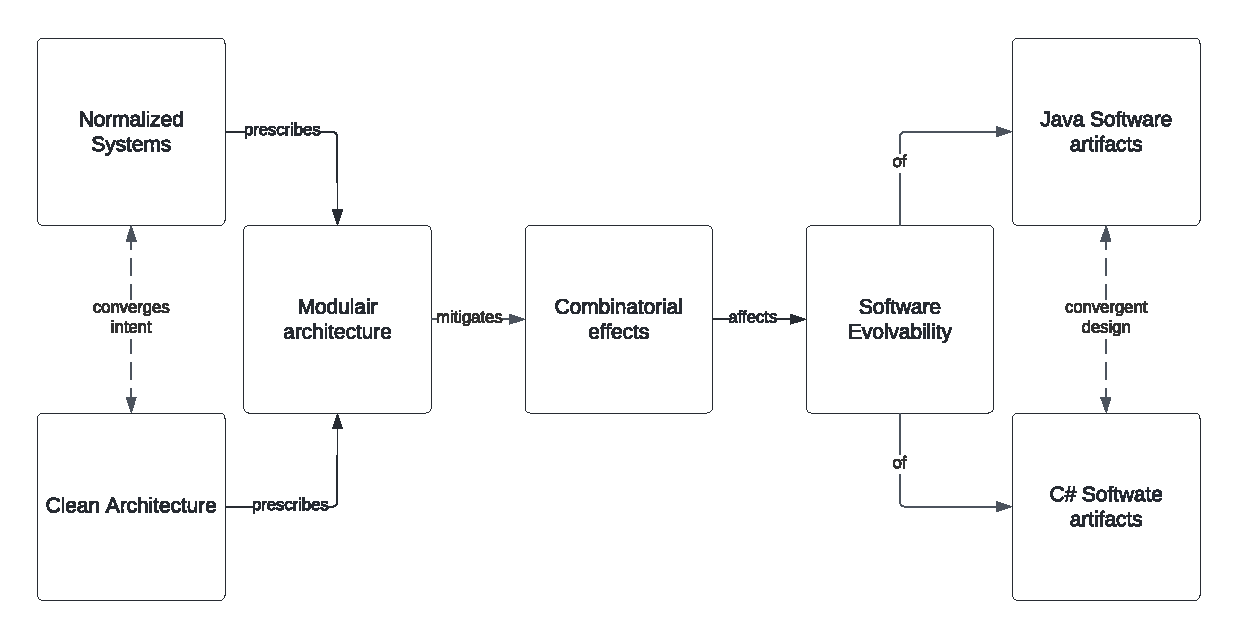
\includegraphics[width=0.9\textwidth]{Figures/hypothesis.pdf}
    \caption[The hypothesis]{The hypothesis}
    \label{fig_hypothesis}
\end{figure}
\section{Research questions} \label{research_questions}
The Hypothesis described in \ref{hypothesis} and \ref{conceptualframework} leads us to the
following research question:

\begin{center}
    \enquote*{\textit{To what extent converges the evolvability of a C\# artifact built
    based on the Clean Architecture principles towards a similar artifact that is based on
    Normalized Systems Theorems?}}
\end{center}

The following sub-questions can be formulated that support the research on the main
research question:
\begin{itemize}
    \item How does Clean Architecture contribute to Software Evolvability?
    \item To what extent Is Normalized Systems applicable to a C\# artifact?   
\end{itemize}
\section{Research model} \label{research_model}

Figure \ref{fig_conceptual_framework} depicts the overall conceptual research framework.
The artifact is the research context. It is a fully functional commerce Restful API with
ASP.NET (v6) and C\# (v10). The research aims to test the cause-and-effect relationship
between Clean Architecture (independent variable) and the evolvability of the C\#
artifact.

The Normalized Systems Theorems do not affect Clean Architecture as an independent
variable. Instead, it will affect the design of the artifact. Previous research and case
studies have already shown that Normalized Systems affect the evolvability of software
artifacts by using a prescribed modular design, mitigating combinatorial effects.
Normalized Systems Theorems is the control variable in the conceptual framework.

Since we are trying to prove the convergence of Normalized Systems and Clean
Architecture the Modular architecture will be compared with the design of Normalized
Systems. Therefore, Modular Architecture is positioned as the Mediator variable in this
conceptual framework.

\begin{figure}[!ht]
    \centering
    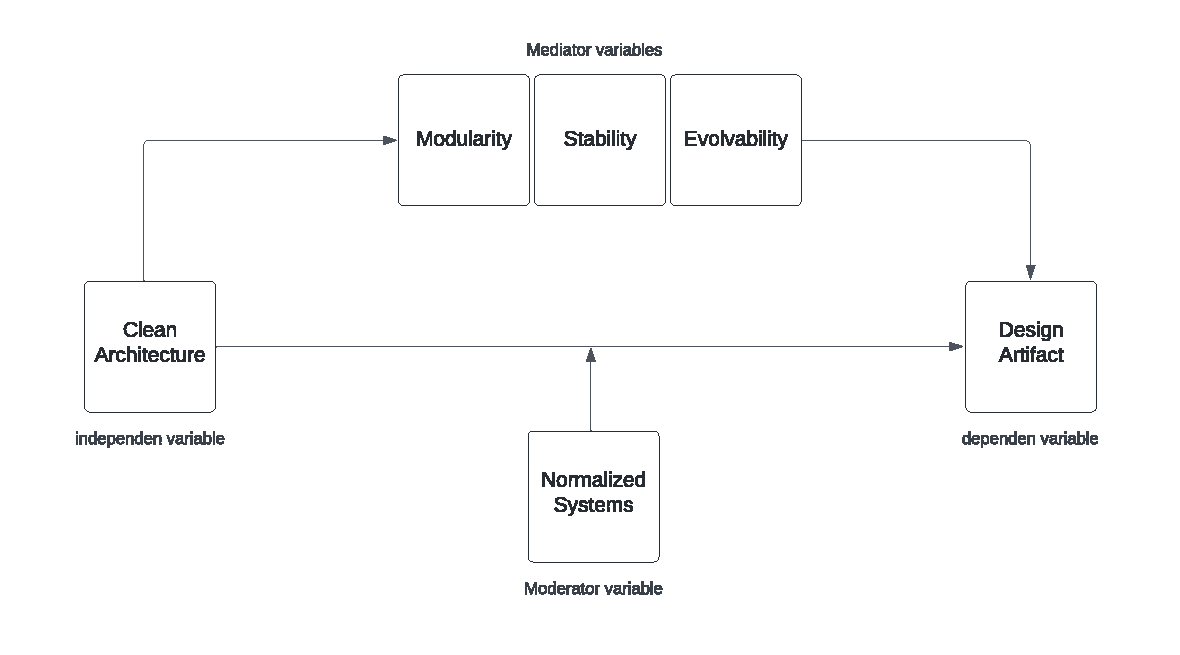
\includegraphics[width=1\textwidth]{Figures/conceptual_framework}
    \caption[Overall conceptual framework]{Overall conceptual framework}
    \label{fig_conceptual_framework}
\end{figure}
